\documentclass{standalone}
%
\usepackage{tikz}
\usetikzlibrary{backgrounds}
\usetikzlibrary{calc}
\usetikzlibrary{decorations.pathmorphing}
\usetikzlibrary{bending,arrows.meta}
\usepackage{xcolor}
%
\definecolor{space}{HTML}{1F2C4E}
\definecolor{earth}{HTML}{0089FA}
\definecolor{mars}{HTML}{DC7B4E}
\definecolor{dida}{HTML}{FFDE00}
\definecolor{title}{HTML}{FBA706}
\definecolor{moon}{HTML}{AFAFAF}
\definecolor{radiation}{HTML}{FFD016}
\definecolor{galaxy}{HTML}{4278A4}
%
\usepackage{fontspec}
\setmainfont{Open Dyslexic}
%
\title{Esopianeti}
\begin{document}
	\tikzset{
		partial ellipse/.style args = {#1:#2:#3}{insert path={+ (#1:#3) arc (#1:#2:#3)}},
		human/.pic = {
			\draw [fill] (0,0) circle (0.3cm);
			\draw [thick] (0,0) circle -- (0,-1.5);
			\draw [thick] (-0.5,-1) -- (0,-0.5) -- (0.5,-1);
			\draw [thick] (-0.5,-2) -- (0,-1.5) -- (0.5,-2);
		},
	}
	\begin{tikzpicture}[background rectangle/.style={fill=white},show background rectangle,>={[inset=0,angle'=27]Stealth}]
		%title
		\draw [black,ultra thick,fill=title] (0,9.8) rectangle (30,16.8);
		\node at (15,14.8) {\textcolor{black}{\fontsize{90}{91}\selectfont Come scoprire}};
		\node at (15,11.8) {\textcolor{black}{\fontsize{90}{91}\selectfont nuovi pianeti}};
		% intro
		\begin{scope}[shift={(0,4)}]
			%dida
			\begin{scope}
				\draw[fill=dida,thick] (11.9,4.2) rectangle (28.2,-4.2);
				\node at (20,3.5) {\textcolor{black}{\fontsize{23}{24}\selectfont La Via Lattea, la nostra galassia,}};
				\node at (20,2.5) {\textcolor{black}{\fontsize{23}{24}\selectfont contiente dai 100 ai 400 miliardi}};
				\node at (20,1.5) {\textcolor{black}{\fontsize{23}{24}\selectfont di stelle. Questo ha spinto gli}};
				\node at (20,0.5) {\textcolor{black}{\fontsize{23}{24}\selectfont astronomi a cercare altre stelle}};
				\node at (20,-0.5) {\textcolor{black}{\fontsize{23}{24}\selectfont con pianeti come compagni.}};
				\node at (20,-1.5) {\textcolor{black}{\fontsize{23}{24}\selectfont La storia di questa ricerca parte da}};
				\node at (20,-2.5) {\textcolor{black}{\fontsize{23}{24}\selectfont una scoperta avvenuta nel 1917 e}};
				\node at (20,-3.5) {\textcolor{black}{\fontsize{23}{24}\selectfont ritrovata nel 2016.}};
			\end{scope}
			% galaxy
			\draw [ultra thick,fill=space] (1,4) rectangle (11.5,-4);
			\begin{scope}[rotate around={30:(6.5,0)}]
				%
				\draw (6.3,0) [dashed,color=galaxy,ultra thick,partial ellipse=0:180:3.2 and 0.7];
				\draw (6.1,0) [dashed,color=galaxy,ultra thick,partial ellipse=0:195:3.4 and 0.8];
				\draw (5.9,0) [dashed,color=galaxy,ultra thick,partial ellipse=0:190:3.6 and 0.9];
				\draw (5.7,0) [dashed,color=galaxy,ultra thick,partial ellipse=0:185:3.8 and 1];
				\draw (5.5,0) [dashed,color=galaxy,ultra thick,partial ellipse=0:200:4 and 1.1];
				%
				\draw [color=galaxy,fill=galaxy!50!white,opacity=0.5,ultra thick] (6.5,0) ellipse (3cm and 0.6cm);
				%
				\draw (6.5,0) [fill=white,ultra thick,partial ellipse=0:180:0.5 and 0.5];
				\draw (6.5,0) [fill=white,ultra thick,partial ellipse=180:360:0.5 and 0.2];
				%	
				\draw (6.7,0) [dashed,color=galaxy,ultra thick,partial ellipse=180:375:3.2 and 0.7];
				\draw (6.9,0) [dashed,color=galaxy,ultra thick,partial ellipse=180:385:3.4 and 0.8];
				\draw (7.1,0) [dashed,color=galaxy,ultra thick,partial ellipse=180:390:3.6 and 0.9];
				\draw (7.3,0) [dashed,color=galaxy,ultra thick,partial ellipse=180:385:3.8 and 1];
				\draw (7.5,0) [dashed,color=galaxy,ultra thick,partial ellipse=180:400:4 and 1.1];
				%
			\end{scope}
		\end{scope}
		%
		\begin{scope}[shift={(0,-4)},decoration=snake]
			\draw [fill=space, ultra thick] (1,3) rectangle (28,-23);
			% Van Maanen
			\node at (8,0) () {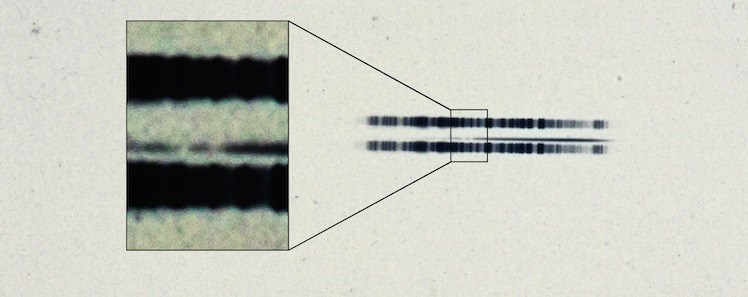
\includegraphics[width=13cm]{img/vanmaanen2.jpg}};
			\draw [fill=dida, thick] (13,2.5) rectangle (29,-2.5);
			\node at (21,2) {\textcolor{black}{\fontsize{17}{18}\selectfont Questo è lo spettro di Van Maanen 2, rilevato}};
			\node at (21,1) {\textcolor{black}{\fontsize{17}{18}\selectfont dall'astronomo \textbf{Adriaan van Maanen} nel 1917.}};
			\node at (21,0) {\textcolor{black}{\fontsize{17}{18}\selectfont Nel 2016 l'astronomo \textbf{Jay Farihi} riesaminando}};
			\node at (21,-1) {\textcolor{black}{\fontsize{17}{18}\selectfont quello spettro dedusse la presenza di un pianeta}};
			\node at (21,-2) {\textcolor{black}{\fontsize{17}{18}\selectfont intorno alla stella di Van Maanen.}};
			% gamma cephei
			\draw [fill=orange] (5,-7) circle (3cm);
			\draw (5,-7) [->,color=galaxy,ultra thick, partial ellipse=310:350:3.5 and 2.3];
			\draw [fill=red] (7,-9) circle (1cm);
			\draw (5,-7) [color=galaxy,ultra thick, partial ellipse=260:295:3.5 and 2.3];
			\draw [fill=dida, thick] (9,-5.5) rectangle (29,-8.5);
			\node at (19,-6) {\textcolor{black}{\fontsize{17}{18}\selectfont Gamma Cephei Ab è il primo esopianeta scoperto: orbita}};
			\node at (19,-7) {\textcolor{black}{\fontsize{17}{18}\selectfont intorno alla stella doppia Gamma Cephei. Scoperto nel 1989,}};
			\node at (19,-8) {\textcolor{black}{\fontsize{17}{18}\selectfont venne confermato solo nel 2002.}};
			% pulsar
			\draw [fill=white] (5,-14) circle (1cm);
			\draw (5,-14) [->,color=galaxy,ultra thick,partial ellipse=200:350:1.5 and 0.5];
			\foreach \x in {-2,-1,0,1,2}
			{\begin{scope}[rotate around={(10 * \x):(5,-14)}]
				\draw [decorate,color=orange,ultra thick] (5,-14+1.2) -- (5,-14+1.5);
				\draw [decorate,color=orange,ultra thick] (5,-14-1.2)-- (5,-14-1.5);
				\end{scope}}
			\draw [fill=dida, thick] (9.5,-12.5) rectangle (26.5,-15.5);
			\node at (18,-13) {\textcolor{black}{\fontsize{17}{18}\selectfont I primi pianeti extrasolari confermati risalgono al}};
			\node at (18,-14) {\textcolor{black}{\fontsize{17}{18}\selectfont 1992 quando venne scoperto un sistema planetario}};
			\node at (18,-15) {\textcolor{black}{\fontsize{17}{18}\selectfont intorno alla pulsar PSR B1257+12.}};
			% Pegasi 51b
			\draw [fill=mars] (5,-20) circle (2.5cm);
			\draw [fill=dida,thick] (9,-17.5) rectangle (27,-22.5);
			\node at (18,-18) {\textcolor{black}{\fontsize{17}{18}\selectfont Nel 1995 \textbf{Michel Mayor} e \textbf{Didier Queloz} scoprirono}};
			\node at (18,-19) {\textcolor{black}{\fontsize{17}{18}\selectfont il primo pianeta extrasolare orbitante intorno a}};
			\node at (18,-20) {\textcolor{black}{\fontsize{17}{18}\selectfont una stella simile al Sole, Pegasi 51.}};
			\node at (18,-21) {\textcolor{black}{\fontsize{17}{18}\selectfont La scoperta è avvenuta utilizzando il metodo della}};
			\node at (18,-22) {\textcolor{black}{\fontsize{17}{18}\selectfont velocità radiale.}};
			%
		\end{scope}
		% radial method
		\begin{scope}[shift={(0,-28.5)}]
			\draw [fill=title] (1,1) rectangle (29,-1);
			\node at (15,0) {\textcolor{black}{\fontsize{23}{24}\selectfont Metodo della velocità radiale}};
		\end{scope}
		%
		\begin{scope}[shift={(0,-40.5)},decoration=snake]
			%
			\draw[fill=space,ultra thick] (2,7.5) rectangle (28,-6.5);
			%
			\draw [fill=dida, thick] (1,10.5) rectangle (29,6.5);
			\node at (15,9.5) {\textcolor{black}{\fontsize{23}{24}\selectfont Non è solo il modo dei pianeti a venire influenzato dalle stelle,}};
			\node at (15,8.5) {\textcolor{black}{\fontsize{23}{24}\selectfont ma anche il moto delle stelle viene influenzato dalla presenza}};
			\node at (15,7.5) {\textcolor{black}{\fontsize{23}{24}\selectfont di pianeti in orbita intorno a esse.}};
			%
			\draw [fill=white] (13,1) circle (2.7cm);
			\draw [ultra thick] (14.8,0.2) -- (15.2,-0.2);
			\draw [ultra thick] (14.8,-0.2) -- (15.2,0.2);
			\draw (15,0) [->,color=galaxy,ultra thick, partial ellipse=245:425:2.2 and 2.2];
			\draw [fill=mars] (20,-3) circle (1cm);
			\draw (15,0) [->,color=galaxy,ultra thick, partial ellipse=-15:315:5.8 and 5.8];
			%
			\draw [fill=dida] (19.8,0.8) rectangle (26,-0.8);
			\draw [fill=white] (15.4,0) -- (15.7,0.3) -- (15.7,0.1) -- (20,0.1) -- (20,-0.1) -- (15.7,-0.1) -- (15.7,-0.3) -- (15.4,0);
			\node at (22.8,0) {\textcolor{black}{\fontsize{17}{18}\selectfont Centro di massa}};
			%
			\draw [fill=dida, thick] (1,-6.5) rectangle (29,-10.5);
			\node at (15,-7.5) {\textcolor{black}{\fontsize{23}{24}\selectfont Questo vuol dire che studiando la luce proveniente da una stella}};
			\node at (15,-8.5) {\textcolor{black}{\fontsize{23}{24}\selectfont è possibile capire se intorno a essa sta orbitando un pianeta}};
			\node at (15,-9.5) {\textcolor{black}{\fontsize{23}{24}\selectfont utilizzando l'effetto Doppler.}};
			%
			\draw (20,-18) [->,color=galaxy,ultra thick, partial ellipse=245:425:2.2 and 2.2];
			\draw (20,-18) [->,color=galaxy,ultra thick, partial ellipse=-15:315:5.8 and 5.8];
			\draw [color=blue, ultra thick,decorate] (18,-17) -- (6,-23);
			\draw [fill=white] (18,-17) circle (2.7cm);
			\draw [ultra thick] (19.8,-17.8) -- (20.2,-18.2);
			\draw [ultra thick] (19.8,-18.2) -- (20.2,-17.8);
			\draw [fill=mars] (25,-21) circle (1cm);
			\draw [fill=earth] (6,-23) circle (2cm);
			%
			\draw [fill=dida, thick] (11,-23) rectangle (29,-26);
			\node at (20,-24) {\textcolor{black}{\fontsize{23}{24}\selectfont Quando una stella si avvicina a noi}};
			\node at (20,-25) {\textcolor{black}{\fontsize{23}{24}\selectfont la luce che emette si sposta verso il blu.}};
			%
			\draw (20,-33) [->,color=galaxy,ultra thick, partial ellipse=110:300:2.2 and 2.2];
			\draw (20,-33) [->,color=galaxy,ultra thick, partial ellipse=165:495:5.8 and 5.8];
			\draw [color=red, ultra thick, decorate] (22,-32) -- (6,-38);
			\draw [fill=white] (22,-32) circle (2.7cm);
			\draw [ultra thick] (19.8,-32.8) -- (20.2,-33.2);
			\draw [ultra thick] (19.8,-33.2) -- (20.2,-32.8);
			\draw [fill=mars] (15,-30) circle (1cm);
			\draw [fill=earth] (6,-38) circle (2cm);
			%
			\draw [fill=dida, thick] (10.5,-38) rectangle (29.5,-41);
			\node at (20,-39) {\textcolor{black}{\fontsize{23}{24}\selectfont Quando una stella si allontana da noi}};
			\node at (20,-40) {\textcolor{black}{\fontsize{23}{24}\selectfont la luce che emette si sposta verso il rosso.}};
		\end{scope}
		%
		\begin{scope}[shift={(0,-90)}]
			%
			\draw [fill=dida,thick] (3.5,7.5) rectangle (26.5,3.5);
			\node at (15,6.5) {\textcolor{black}{\fontsize{23}{24}\selectfont L'effetto Doppler è quel fenomeno alla base della}};
			\node at (15,5.5) {\textcolor{black}{\fontsize{23}{24}\selectfont diminuzione o dell'aumento di volume del suono di}};
			\node at (15,4.5) {\textcolor{black}{\fontsize{23}{24}\selectfont una sirena in allontanamento o in avvicinamento.}};
			\draw (15,0) [fill=red,thick, partial ellipse=0:180:1 and 2];
			\draw (15,0) [fill=red,thick, partial ellipse=180:360:1 and 0.2];
			\draw [fill=red!50!white,rotate around={15:(15.5,1.3)}] (15.5,1.3) ellipse (0.2cm and 0.5cm);
			\draw [->,ultra thick] (14.5,-0.5) -- (15.5,-0.5);
			\foreach \x in {0,0.5,...,11}
			\draw (16.5 + \x,1) [ultra thick, color=blue, partial ellipse=-90:90:0.2 and 1];
			\foreach \x in {0,1,...,11}
			\draw (13.5 - \x,1) [ultra thick, color=red, partial ellipse=90:270:0.2 and 1];
			\pic at (4,-1) {human};
			\pic at (26,-1) {human};
		\end{scope}
		% method transition
		\begin{scope}[shift={(0,-95)}]
			\draw [fill=title] (1,1) rectangle (29,-1);
			\node at (15,0) {\textcolor{black}{\fontsize{23}{24}\selectfont Metodo del transito}};
		\end{scope}
		%
		\begin{scope}[shift={(0,-102.5)}]
			\draw [fill=space,ultra thick] (1,6) rectangle (29,-7.5);
			%
			\draw (15,0) [->,color=galaxy,ultra thick, partial ellipse=100:125:13 and 1.8];
			\draw (15,0) [color=galaxy,ultra thick, partial ellipse=120:135:13 and 1.8];
			\draw (15,0) [color=galaxy,ultra thick, partial ellipse=45:80:13 and 1.8];
			\draw (15,0) [->,color=galaxy,ultra thick, partial ellipse=325:410:13 and 1.8];
			\draw [fill=radiation] (15,0) circle (5cm);
			\draw [fill=mars] (5,1) circle (1cm);
			\draw [fill=mars] (25,-1) circle (1cm);
			\draw (15,0) [->,color=galaxy,ultra thick, partial ellipse=145:240:13 and 1.8];
			\draw (15,0) [->,color=galaxy,ultra thick, partial ellipse=230:300:13 and 1.8];
			\draw (15,0) [color=galaxy,ultra thick, partial ellipse=290:320:13 and 1.8];
			\draw [fill=mars] (15,-1.8) circle (1cm);
			%
			\draw [color=moon,fill=black,ultra thick] (1.2,-6.5) rectangle (28.8,-9);
			\draw [ultra thick,color=white] (1.5,-7) -- (9.8,-7) to[out=0,in=90] (10,-7.2) -- (10,-8.3) to[out=270,in=180] (10.2,-8.5) -- (19.8,-8.5) to[out=0,in=270] (20,-8.3) -- (20,-7.2) to[out=90,in=180] (20.2,-7) -- (28.5,-7);
			%
			\draw [fill=dida, thick] (0.5,-10) rectangle (29.5,-16);
			\node at (15,-11) {\textcolor{black}{\fontsize{23}{24}\selectfont Quando un pianeta passa davanti a una stella, ovvero "transita"}};
			\node at (15,-12) {\textcolor{black}{\fontsize{23}{24}\selectfont di fronte a essa, la quantità di luce emessa dalla stella diminuisce.}};
			\node at (15,-13) {\textcolor{black}{\fontsize{23}{24}\selectfont Questo vuol dire che, studiando la curva di luce della stella (vedi}};
			\node at (15,-14) {\textcolor{black}{\fontsize{23}{24}\selectfont sopra) è possibile determinare se intorno a quella determinata}};
			\node at (15,-15) {\textcolor{black}{\fontsize{23}{24}\selectfont stella sta orbitando un pianeta o no.}};
		\end{scope}
		% kepler
		\begin{scope}[shift={(0,-125)}]
			\draw [fill=space,thick] (1,5) rectangle (29,1);
			%
			\draw [color=space,fill=white,ultra thick] (3.5,1.6) -- (8.4,-6.95) -- (10.9,-6.92) -- (12.9,-5) -- (12.1,-3.4) -- (7,4.7) -- (3.5,1.6);
			\draw [color=space,ultra thick] (12.1,-3.4) -- (11.5,-3.4);
			\draw [color=space,fill=moon,ultra thick] (3.35,4.3) -- (8.5,-4.9) to[out=-60,in=300] (11.6,-2.8) -- (7.8,3.9) to[out=130,in=130] (3.35,4.3);
			\draw [color=space,fill=white,ultra thick] (3.5,1.6) -- (7.5,-5.4) -- (10.1,-5.35) -- (9.9,-5) -- (3.7,1.7) -- (3.5,1.6);
			\draw [color=space,ultra thick] (12.1,-3.4) -- (10.1,-5.35) -- (10.9,-6.92);
			%
			\node at (20,4) {\textcolor{white}{\fontsize{23}{24}\selectfont Il satellite Kepler, in 9 anni di attività,}};
			\node at (19.1,3) {\textcolor{white}{\fontsize{23}{24}\selectfont ha scoperto oltre 4100 pianeti extrasolari}};
			\node at (19.2,2) {\textcolor{white}{\fontsize{23}{24}\selectfont utilizzando proprio il metodo del transito.}};
		\end{scope}
		%
		\begin{scope}[shift={(0,-134)}]
			\node at (27,0) () {
\includegraphics[width=3.7cm]{licenza}};
			\node at (18,-0.1) {\textcolor{black}{\fontsize{14}{15}\selectfont Testo e illustrazioni: @ulaulaman - Gianluigi Filippelli}};
		\end{scope}
	\end{tikzpicture}
%
\end{document}
